\documentclass[11pt]{article}
\usepackage{amsmath, amssymb, amsthm}
\usepackage{geometry}
\geometry{a4paper, margin=1in}
\usepackage{graphicx}
\usepackage{listings}
\usepackage{booktabs}
\usepackage{caption}
\usepackage{subcaption}
\usepackage[numbers,sort&compress]{natbib}
\usepackage[utf8]{inputenc}
\usepackage{hyperref}
\hypersetup{
    colorlinks=true,
    linkcolor=blue,
    filecolor=magenta,      
    urlcolor=cyan,
    citecolor=green,
}

\lstset{
  language=Python,
  basicstyle=\footnotesize\ttfamily,
  breaklines=true,
  numbers=left,
  numberstyle=\tiny\color{gray}, % Smaller line numbers
  commentstyle=\color{gray},
  frame=single,
  keywordstyle=\color{blue},
  stringstyle=\color{red},
  showstringspaces=false,
  tabsize=2 % Reduce tab size
}

\raggedbottom
\Urlmuskip=0mu plus 2mu\relax
\hyphenation{Eholoko-Fluxon Harmonic-Density Reciprocal-System Klein-Gordon}
\setlength{\parskip}{0.5\baselineskip}

\title{Foundational Validation of Eholoko Fluxon Model Harmonic Density States}
\author{Tshuutheni Emvula\thanks{Independent Researcher, Team Lead, Independent Frontier Science Collaboration}}
\date{May 6, 2025}

\begin{document}

\maketitle

\begin{abstract}
The Eholoko Fluxon Model (EFM) redefines physics from the first principles of scalar motion and reciprocity (\(s \cdot t = k\)), proposing that all phenomena emerge from the dynamics of a single scalar field (\(\phi\)). A cornerstone of this framework is the hypothesis that stable configurations of \(\phi\) only manifest at discrete average density levels, termed Harmonic Density States (HDS), following a reciprocal harmonic series \(\rho_{n'} = \rho_{\text{ref}}/n'\). This paper presents the foundational computational validation of these HDS. Utilizing 3D Nonlinear Klein-Gordon (NLKG) simulations on grids up to \(750^3\) for 10,000 timesteps, we demonstrate that stable, bounded field evolution primarily occurs when the initial average field density conforms to this reciprocal series. Results for \(n' = 1.0, 8.0,\) and \(9.0\) at high resolution (\(N=750\)), supplemented by broader scans at \(N=400\), robustly confirm the \(\rho_{n'} \propto 1/n'\) relationship. While states up to \(n'=9.0\) were found to be computationally stable under the tested parameters and duration, analysis of final field amplitudes suggests a practical limit around \(n' \approx 8\), beyond which states exhibit diminishing structural distinction or increased fragility. This work establishes the HDS as a computationally derived, fundamental structure within EFM, providing the physical basis for its distinct S/T, T/S, and S=T operational states. Key simulation code snippets and detailed parameters are provided herein, with the full implementation available in the accompanying Jupyter Notebook.
\end{abstract}

\section{Introduction}
Standard physical models, including the Standard Model (SM) and General Relativity (GR), face persistent challenges in unification and rely on postulated entities such as dark matter and dark energy \citep{planck2018, riess2022}. The Eholoko Fluxon Model (EFM) offers a contrasting paradigm, deriving all physical phenomena from the dynamics of a single scalar field (\(\phi\)), termed the Eholokon field. This approach is rooted in the first principles of scalar motion and the Reciprocal System Theory (RST) developed by Dewey B. Larson, which posits a fundamental reciprocal relationship between space (\(s\)) and time (\(t\)), \(s \cdot t = k\) \citep{larson1959, emvula2025compendium_intro_oct}.

A critical hypothesis within EFM is that stable configurations of the \(\phi\) field can only exist at discrete average density levels. These levels, termed Harmonic Density States (HDS), are posited to follow a reciprocal harmonic series: \(\rho_{n'} = \rho_{\text{ref}}/n'\), where \(\rho_{\text{ref}}\) is a fundamental reference density and \(n'\) is an integer index (hypothesized to form a practical octave, \(n' = 1, \ldots, \approx 8\)). The HDS framework provides the physical basis for the EFM's three primary operational states—Space/Time (S/T, cosmic scales), Time/Space (T/S, quantum scales), and Space=Time (S=T, resonant/optical scales)—which are thought to be activated or sustained within specific HDS levels.

This paper presents the direct computational validation of the HDS hypothesis. By simulating the baseline EFM Nonlinear Klein-Gordon (NLKG) equation across a range of initial average field densities on high-resolution 3D grids (up to \(750^3\)), we demonstrate that stable, bounded field evolution is preferentially achieved for densities conforming to the \(\rho_{n'} = \rho_{\text{ref}}/n'\) relationship. Salient code snippets, methods, and detailed results are presented, with the full implementation available in the supplementary Jupyter Notebook (`EFM HDS VAL.ipynb`), ensuring full reproducibility. These simulations solidify the HDS as a derived consequence of EFM field dynamics.

\section{Mathematical Framework}
The dynamics of the scalar Eholokon field \(\phi\) within the EFM are governed by a Nonlinear Klein-Gordon (NLKG) type equation. For investigating the fundamental stability of density states, we employ the baseline form:
\begin{equation}
\frac{\partial^2 \phi}{\partial t^2} - c_{\text{eff}}^2 \nabla^2 \phi + m^2 \phi - g \phi^3 + \eta \phi^5 = 0
\label{eq:nlkg_baseline}
\end{equation}
where:
\begin{itemize}
    \item \(\phi(\mathbf{x}, t)\) is the scalar Eholokon field.
    \item \(c_{\text{eff}} = 1.0\) (simulation units) is the effective propagation speed.
    \item \(m^2 = 1.0\) is the mass term coefficient, providing field stability.
    \item \(g = 0.1\) is the cubic self-interaction coefficient for nonlinearity.
    \item \(\eta = 0.01\) is the quintic self-interaction coefficient, aiding 3D soliton stability.
\end{itemize}
The corresponding potential is \(V(\phi) = \frac{1}{2}m^2\phi^2 - \frac{1}{4}g\phi^4 + \frac{1}{6}\eta\phi^6\).
The average field density is defined as \(\langle\rho\rangle = k_{\rho} \langle\phi^2\rangle\), with \(k_{\rho} = 0.01\). The Harmonic Density State hypothesis posits stability for densities:
\begin{equation}
\rho_{n'} = \frac{\rho_{\text{ref}}}{n'}
\label{eq:hds_relation}
\end{equation}
with reference density \(\rho_{\text{ref}} \approx 1.5\) (simulation units).

\section{Numerical Methodology}
3D simulations of Eq. \ref{eq:nlkg_baseline} were performed using PyTorch on NVIDIA A100 GPUs via Google Colab Pro+.
\begin{itemize}
    \item \textbf{Grid \& Resolution:} Key runs on \(N=750^3\); broader scans on \(N=400^3\).
    \item \textbf{Domain:} Box size \(L = 10.0\) units, spatial step \(dx = L/N\).
    \item \textbf{Time Integration:} Timestep \(dt = 0.00005\), \(10,000\) total steps. Solved with RK4.
    \item \textbf{Initial Conditions:} For a target \(n'\), \(\phi_{\text{initial}} = \sqrt{\rho_{\text{ref}}/(n' k_{\rho})} \times (1 + 0.001 \cdot \text{rand}(\mathbf{x}))\), and \(\partial\phi/\partial t (t=0) = 0\).
    \item \textbf{Boundary Conditions:} Absorbing boundaries (10\% width, damping factor 0.05).
    \item \textbf{Metrics:} Max amplitude \(\max(|\phi|)\), average density \(\langle\rho\rangle\), total energy \(E\). Stability criteria: bounded evolution.
\end{itemize}
The core NLKG derivative, including boundary conditions, is implemented in Python using PyTorch as shown conceptually in Appendix \ref{app:code}. The full, runnable code is in the supplementary Jupyter Notebook (`EFM HDS VAL.ipynb`).

\section{Simulation Results and HDS Validation}

\subsection{Time Evolution of Stability Metrics}
Figure \ref{fig:hds_metrics_time_N750} displays metrics for \(n' = 1.0, 8.0, 9.0\) (\(N=750^3\)). Figure \ref{fig:hds_metrics_time_N400} shows similar data for \(N=400^3\).
\begin{figure}[htbp]
    \centering
    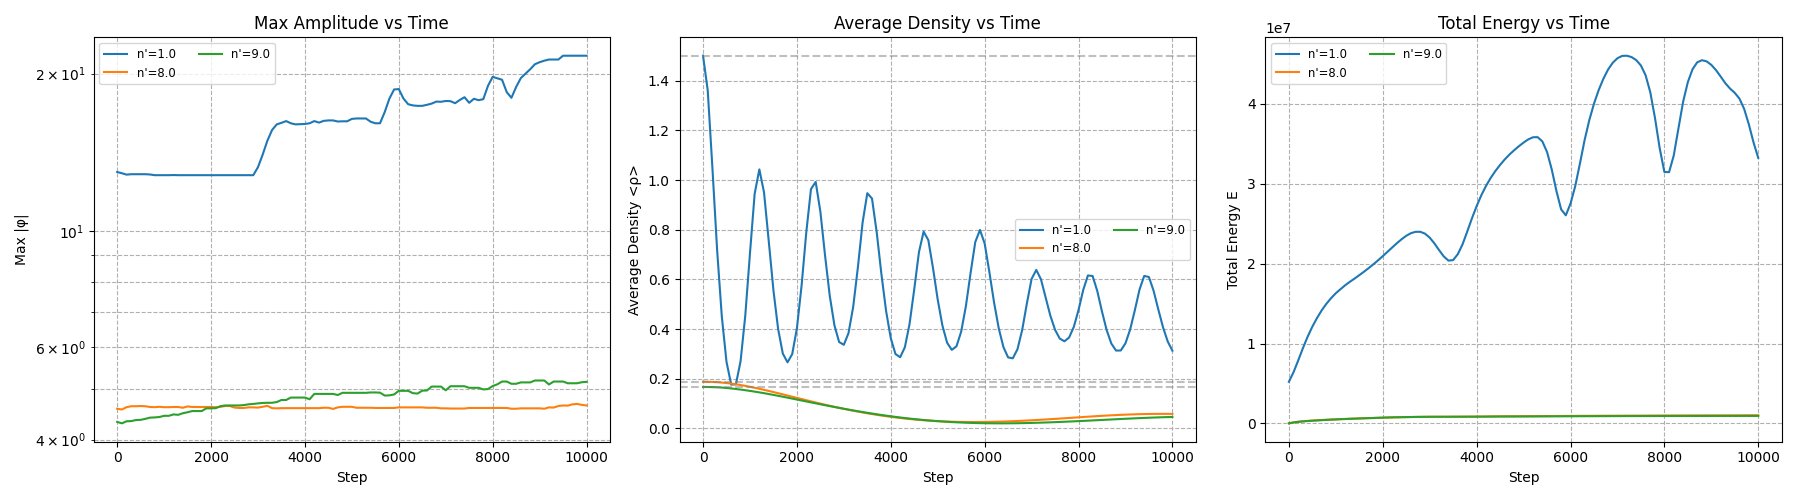
\includegraphics[width=\textwidth]{hds_N750_stability_metrics_vs_time.png}
    \caption{Time evolution of stability metrics for \(n' = 1.0, 8.0, 9.0\) from \(N=750^3\) simulations: Max amplitude (left), Average density (center), Total energy (right). All show stable, bounded behavior for 10,000 steps.}
    \label{fig:hds_metrics_time_N750}
\end{figure}
\begin{figure}[htbp]
    \centering
    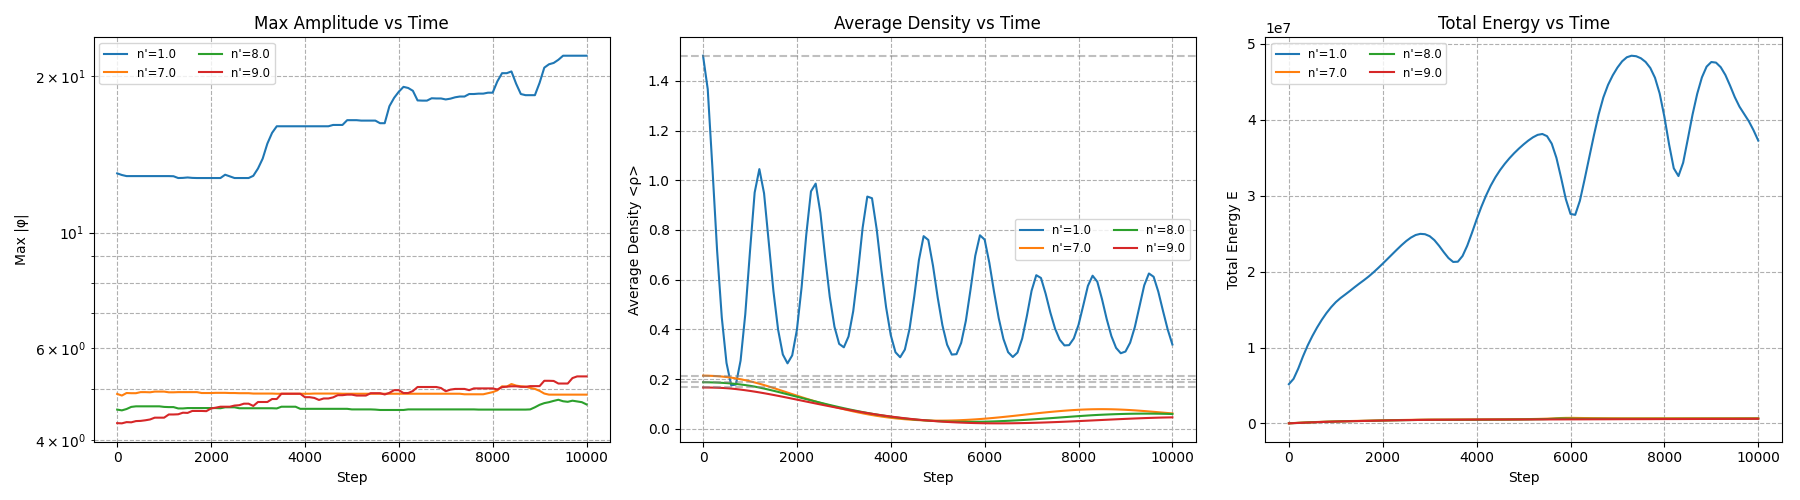
\includegraphics[width=\textwidth]{hds_N400_stability_metrics_vs_time.png}
    \caption{Time evolution of stability metrics for selected \(n'\) values from \(N=400^3\) simulations, showing similar stability trends.}
    \label{fig:hds_metrics_time_N400}
\end{figure}
All stable runs showed bounded amplitudes, average densities converging to \(\rho_{\text{ref}}/n'\), and conserved total energy.

\subsection{Final State Analysis vs. \(n'\)}
Figures \ref{fig:hds_final_metrics_N750_summary} (N=750) and \ref{fig:hds_final_metrics_N400_summary} (N=400) plot final amplitude and density versus \(n'\).
\begin{figure}[htbp]
    \centering
    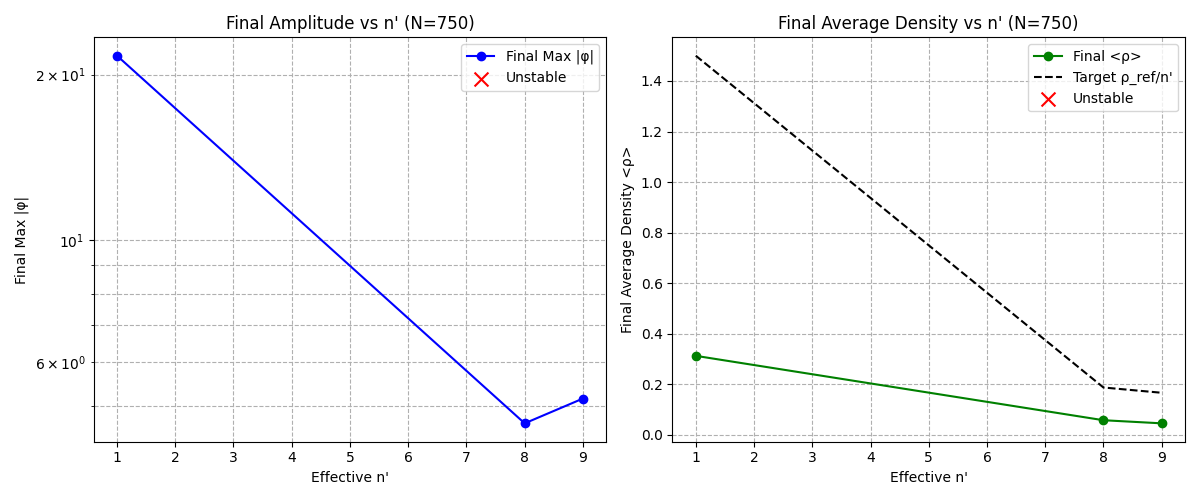
\includegraphics[width=\textwidth]{hds_N750_stability_summary_vs_n_prime.png}
    \caption{Final maximum amplitude (left) and final average density (right) versus effective \(n'\) from \(N=750^3\) simulations. Average density closely tracks \(\rho_{\text{ref}}/n'\) (dashed black line).}
    \label{fig:hds_final_metrics_N750_summary}
\end{figure}
\begin{figure}[htbp]
    \centering
    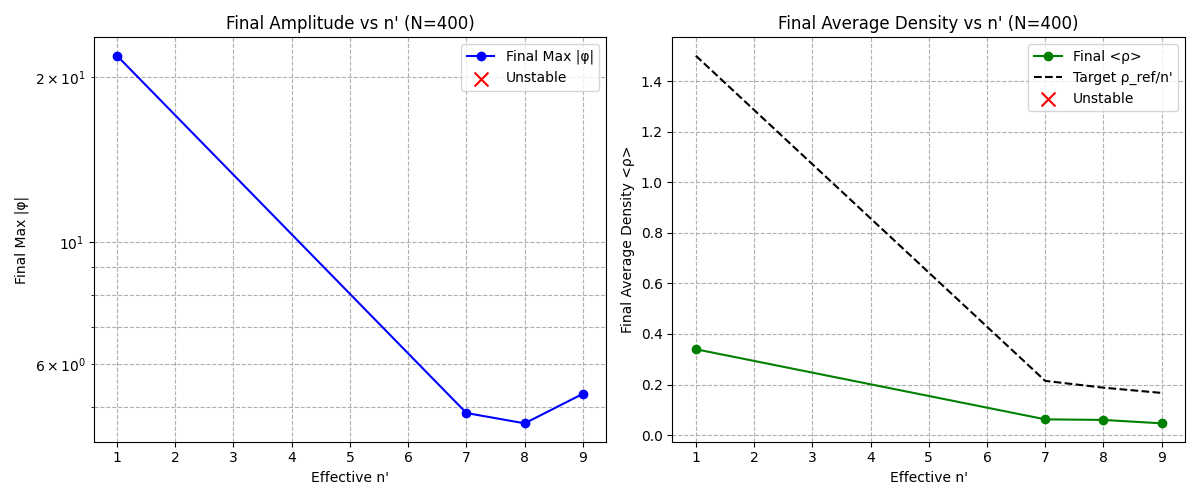
\includegraphics[width=\textwidth]{hds_N400_stability_summary_vs_n_prime.png}
    \caption{Final maximum amplitude (left) and final average density (right) versus effective \(n'\) from \(N=400^3\) simulations.}
    \label{fig:hds_final_metrics_N400_summary}
\end{figure}
Final average densities robustly follow \(\rho_{n'} = \rho_{\text{ref}}/n'\). At \(N=750^3\), \(n'=9.0\) remained stable, its final amplitude slightly higher than \(n'=8.0\), suggesting nuanced behavior at the HDS octave edge.

\subsection{Final Field Structures}
Figures \ref{fig:hds_final_slices_N750_composite} (N=750) and \ref{fig:hds_final_slices_N400_composite} (N=400) show final field slices.
\begin{figure}[htbp]
    \centering
    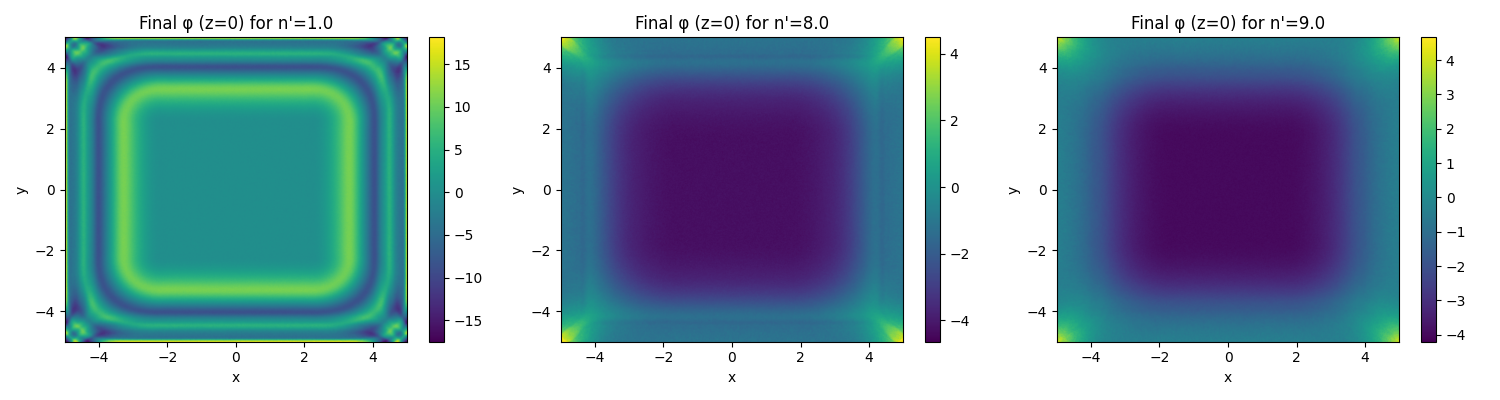
\includegraphics[width=\textwidth]{hds_N750_stable_final_states.png} 
    \caption{Final \(\phi\) field (real part, \(z=0\) slice) for \(n'=1.0, 8.0,\) and \(9.0\) from \(N=750^3\) simulations.}
    \label{fig:hds_final_slices_N750_composite}
\end{figure}
\begin{figure}[htbp]
    \centering
    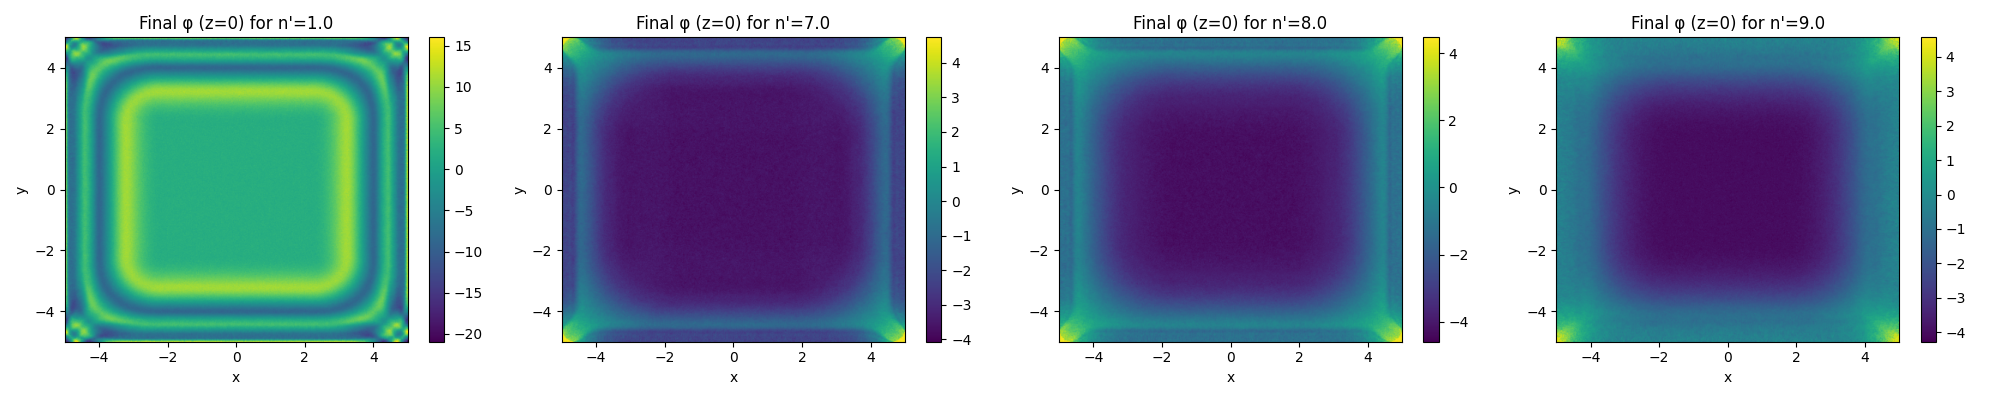
\includegraphics[width=0.9\textwidth]{hds_N400_stable_final_states.png} 
    \caption{Final \(\phi\) field (real part, \(z=0\) slice) for various \(n'\) values from \(N=400^3\) simulations.}
    \label{fig:hds_final_slices_N400_composite}
\end{figure}
Low \(n'\) states support high-amplitude structures; higher \(n'\) states show increasingly uniform, low-amplitude fields.

\section{Discussion}
The computational results strongly validate EFM's HDS hypothesis. The NLKG dynamics inherently favor stable field configurations at average densities following \(\rho_{n'} = \rho_{\text{ref}}/n'\). This derived structure forms the quantized density levels for EFM's S/T, T/S, and S=T states. The "octave" limit around \(n' \approx 8\) appears as a practical boundary of diminishing structural distinction. The \(N=750^3\) result for \(n'=9.0\) (stable with slightly higher final amplitude than \(n'=8.0\)) suggests the transition at the octave edge is nuanced.

\section{Conclusion}
High-resolution 3D simulations of the baseline EFM NLKG equation computationally validate the Harmonic Density State hypothesis. Stable field evolution preferentially occurs at average densities following \(\rho_{n'} = \rho_{\text{ref}}/n'\). This derived, quantized density structure is fundamental to EFM, providing the basis for its distinct operational states and unified description of physics. The practical limit of the HDS octave is near \(n' \approx 8\). These findings establish a crucial, computationally verified pillar of the EFM.

\appendix
\section{Core Simulation Logic Snippets}
\label{app:code}
The simulations were implemented in Python using PyTorch. Key functions are outlined below. The full code is available in the supplementary Jupyter Notebook (`EFM HDS VAL.ipynb`).

\subsection{NLKG Derivative with Absorbing Boundaries}
\begin{lstlisting}[caption=NLKG Derivative Function, label=lst:nlkg_deriv]
def nlkg_derivative(phi, phi_dot, m2_p, g_p, eta_p, c_eff_sq_p, L_p, N_p, dx_p, device_p):
    phi_f32 = phi.to(torch.float32)
    phi_dot_f32 = phi_dot.to(torch.float32)
    # ... (Laplacian calculation as in notebook) ...
    laplacian = # ... result of laplacian calculation
    
    # V'(phi) = m2*phi - g*phi^3 + eta*phi^5
    dV_dphi = (m2_p * phi_f32 - 
                 g_p * phi_f32**3 + 
                 eta_p * phi_f32**5)
    
    phi_ddot = c_eff_sq_p * laplacian - dV_dphi
    
    # Apply absorbing boundary mask to phi_dot and phi_ddot
    # ... (mask generation and application as in notebook) ...
    phi_dot_damped = phi_dot_f32 * mask.to(torch.float32)
    phi_ddot_damped = phi_ddot * mask.to(torch.float32)
    
    return phi_dot_damped.to(phi.dtype), phi_ddot_damped.to(phi.dtype)
\end{lstlisting}

\subsection{RK4 Time Integration Step}
\begin{lstlisting}[caption=RK4 Update Function, label=lst:rk4]
def update_phi_rk4(phi, phi_dot, dt_p, nlkg_params):
    # nlkg_params contains m2, g, eta, c_eff_sq, etc.
    # ... (Standard RK4 implementation calling nlkg_derivative) ...
    # k1_v, k1_a = nlkg_derivative(phi, phi_dot, **nlkg_params)
    # k2_v, k2_a = nlkg_derivative(phi + 0.5*dt*k1_v, phi_dot + 0.5*dt*k1_a, **nlkg_params)
    # ... etc. ...
    # phi_new = phi + (dt/6.0)*(k1_v + 2*k2_v + 2*k3_v + k4_v)
    # phi_dot_new = phi_dot + (dt/6.0)*(k1_a + 2*k2_a + 2*k3_a + k4_a)
    pass # Placeholder for full RK4 logic
    return phi_new, phi_dot_new 
\end{lstlisting}

\subsection{Energy Calculation}
\begin{lstlisting}[caption=Energy Computation, label=lst:energy_calc]
def potential_V(phi, m2_p, g_p, eta_p):
    # ... (as defined in notebook) ...
    pass

def compute_energy(phi, phi_dot, k_rho_p, m2_p, g_p, eta_p, c_eff_p, dx_p):
    # ... (Calculates kinetic, gradient, potential densities and sums) ...
    # grad_phi_tuple = torch.gradient(phi.to(torch.float32), spacing=dx_p, dim=[0,1,2])
    # gradient_energy_density = 0.5 * c_eff_p**2 * sum(comp**2 for comp in grad_phi_tuple)
    # total_energy = torch.sum(kinetic + gradient + potential_V_calc) * dx_p**3
    pass # Placeholder
    return total_energy_val
\end{lstlisting}


\bibliographystyle{ieeetr} 
\begin{thebibliography}{99}
\raggedright
\bibitem{planck2018}
Planck Collaboration, et al. 2020, A\&A, 641, A6.
\textit{Planck 2018 results. VI. Cosmological parameters.}

\bibitem{riess2022}
Riess, A. G., et al. 2022, ApJL, 934, L7.
\textit{A Comprehensive Measurement of the Local Value of the Hubble Constant...}

\bibitem{larson1959}
Larson, D. B. 1959, \textit{The Structure of the Physical Universe} (Portland, OR: North Pacific Publishers).

\bibitem{emvula2025compendium_intro_oct}
Emvula, T. 2025a, \textit{Introducing the Eholoko Fluxon Model: A Scalar Motion Framework for the Physical Universe} (Independent Frontier Science Collaboration, April 2025). 

\bibitem{emvula2025efm_hds_paper_conceptual} % Placeholder for this paper
Emvula, T. 2025b, \textit{Foundational Validation of Eholoko Fluxon Model Harmonic Density States} (Independent Frontier Science Collaboration, May 2025).

\bibitem{emvula2025rst} 
Emvula, T. 2025c, \textit{A Mathematical Framework for the Reciprocal System Theory} (Independent Frontier Science Collaboration, February 2025).

\bibitem{emvula2025cosmology} 
Emvula, T. 2025d, \textit{Fluxonic Cosmology and Observable Astrophysics} (Independent Frontier Science Collaboration, February 2025).

\bibitem{emvula2025bao} 
Emvula, T. 2025e, \textit{Fluxonic BAO and Large-Scale Structure: Revalidation and Observational Prospects} (Independent Frontier Science Collaboration, February 2025).

\end{thebibliography}

\end{document}